\section{Calibration of the NaI Scintilator}

Calibration of the NaI-scintilator was done analogous to the HPGE.
We used the same probes, exept for a new $^{22}$Na source, instead of $^{152}$Eu for another full energy peak analysis.
The probes were changed, because of the lower resolution fg the scintilator.

For this measurement we took a new measurement of the background radiation with the scintilator (see Fig. \ref{back_nai}.

\begin{figure}[h]
  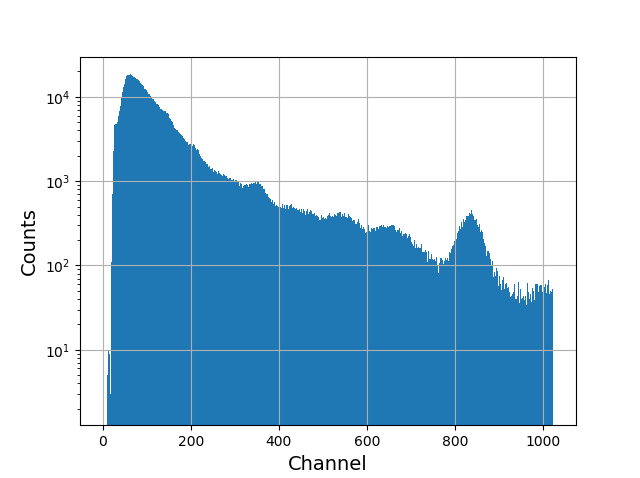
\includegraphics[width=\linewidth]{pictures/szin_background.png}
  \caption{Background radiation measured with the NaI scintilator}
  \label{nai_untergrund}
\end{figure}

This background was again substracted from every measured spectrum.
The measured spectra can be seen in Fig. \ref{szin}.
Just from looking at the spectra, we can already see that this scintilator has a much lower resolution.
The energy of the peaks were again taken from (iaea einfügen).
One special case here is with the $^{22}$Na sample.
In this spectrum we can't see any good gamma peaks.
The one we used, with an energy of $511$ keV has it's origin in photons that are created by annihilation of electrons und positrons, which are created by beta decay of $^{22}$N.

\begin{figure}[h]
\begin{subfigure}{.5\textwidth}
  \centering
  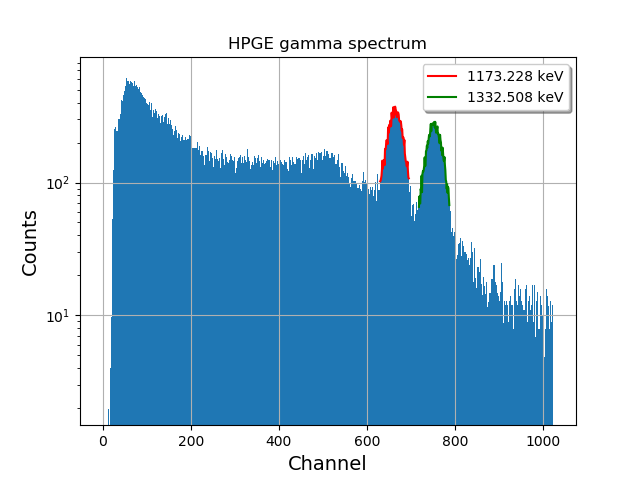
\includegraphics[width=.9\linewidth]{pictures/szin_co.png}
  \caption{$^{60}\text{Co}$}
\end{subfigure}%
\begin{subfigure}{.5\textwidth}
  \centering
  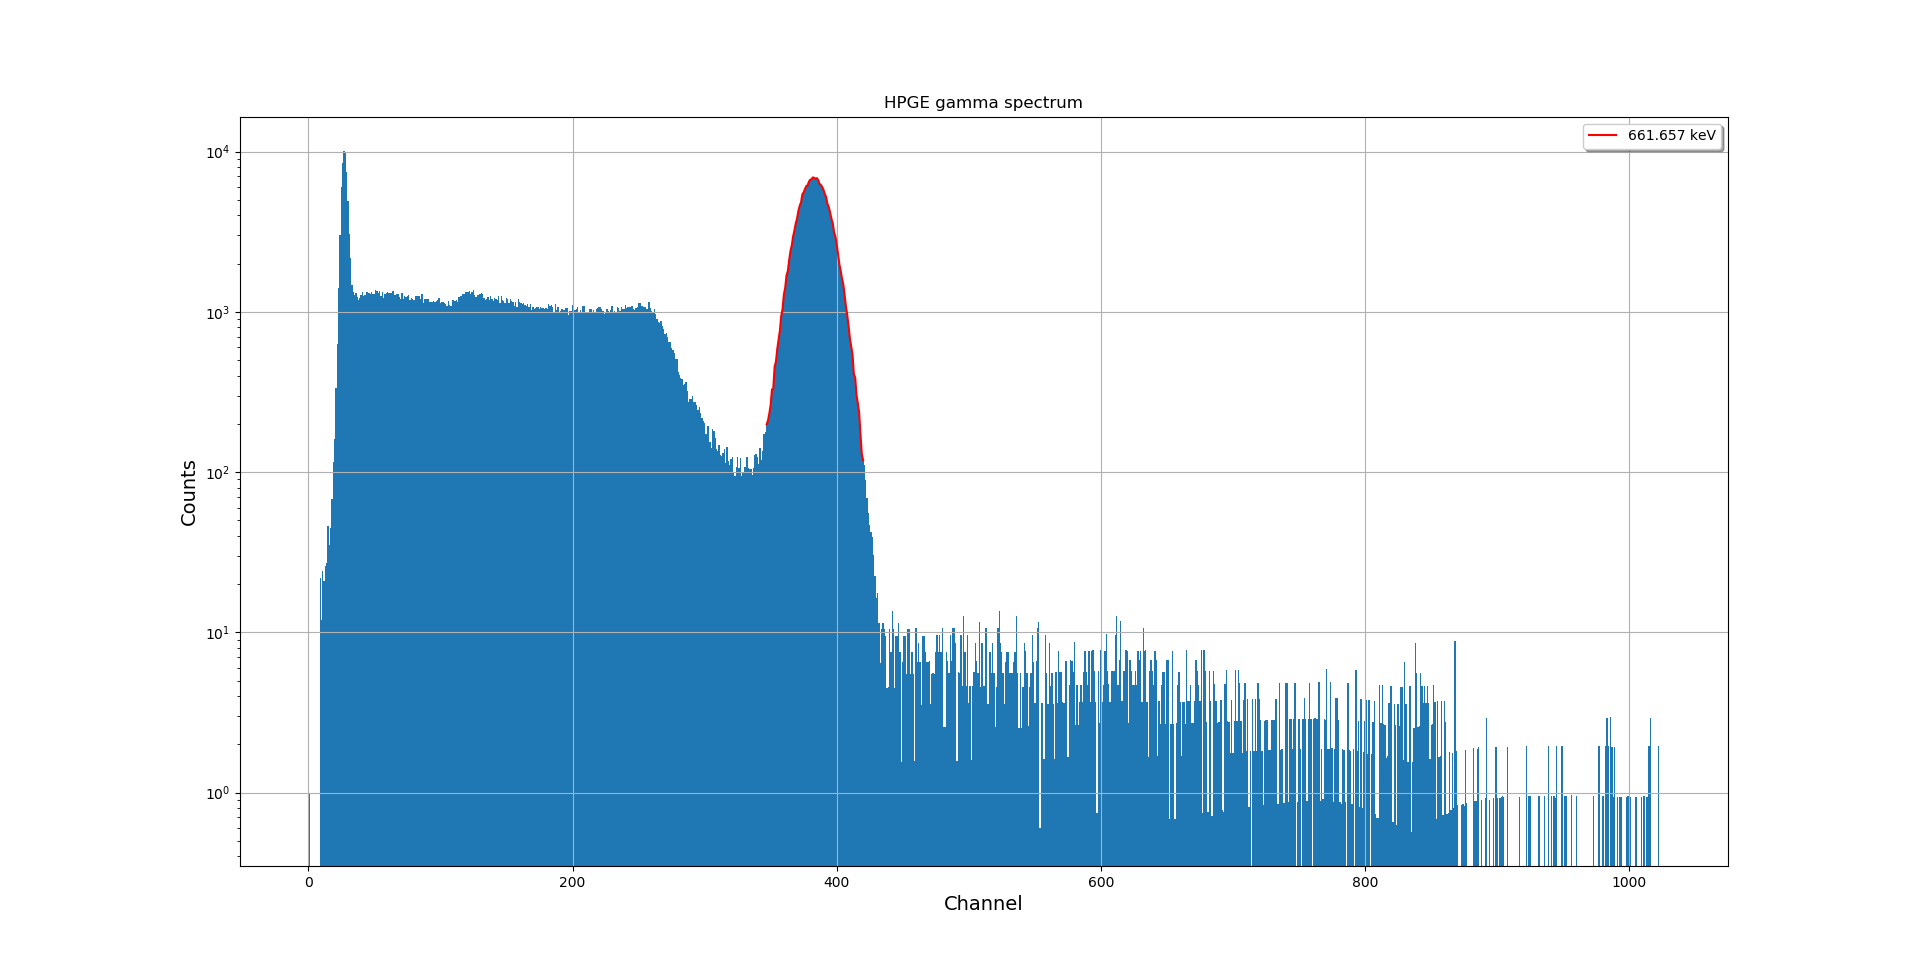
\includegraphics[width=.9\linewidth]{pictures/szin_cs.png}
  \caption{$^{137}\text{Cs}$}
\end{subfigure}%
 \vskip\baselineskip
\begin{subfigure}{.5\textwidth}
  \centering
  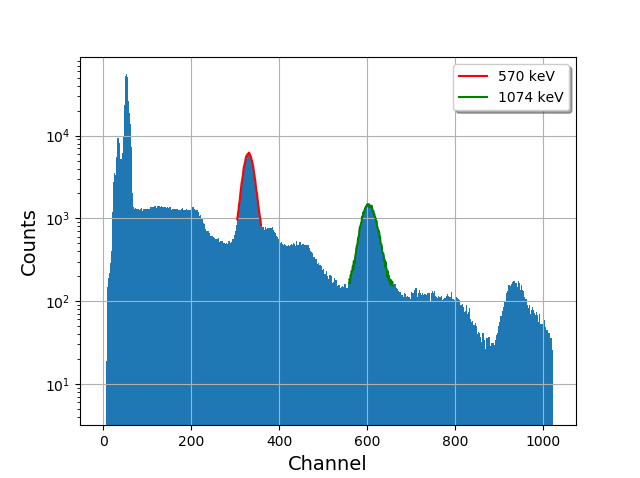
\includegraphics[width=.9\linewidth]{pictures/szin_bi.png}
  \caption{$^{207}\text{Ba}$}
\end{subfigure}%
\begin{subfigure}{.5\textwidth}
  \centering
  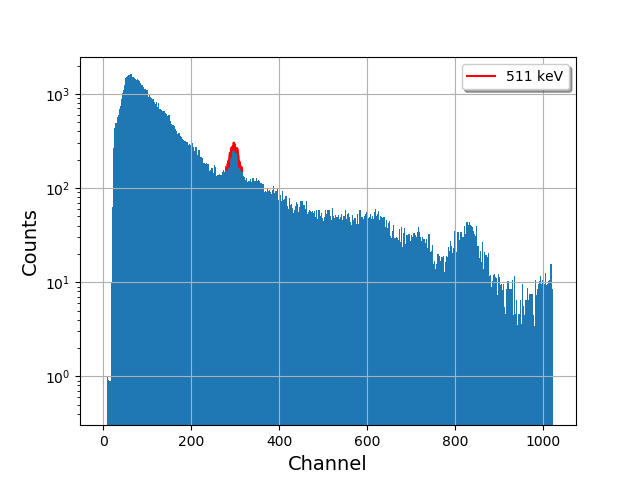
\includegraphics[width=.9\linewidth]{pictures/szin_na.png}
  \caption{$^{22}\text{Na}$}
\end{subfigure}%
\caption{gamma spectra of the measured sources}
\label{szin}
\end{figure}

We fitted the marked peaks again with a guassian function:
\begin{equation}
N(K) = a \cdot exp \left( - \frac{(K - K_{0}^{2}}{2 \sigma ^{2}} \right)
\end {equation}
Where $N$ are the counts and $K$ are the channels.
This gave us channels correspondig to a energy and the FHWM as measure of uncertainty.
The results can be seen in Tab, \ref{szin_peaks}.

\begin{table}[h]
\centering
\begin{tabular}{c |c | c |c}
\hline
Isotop & $E_{\gamma}$ [keV]  & Channel & FWHM \\
\hline
$^{137}Cs$ & $661.7$ & 383 & 29 \\
$^{60}Co$ & $1173.2$ & 664 & 27 \\
$^{60}Co$ & $1332.5$ & 753 & 39 \\
$^{207}Bi$ & $569.7$   & 331 & 27 \\
$^{207}Bi$ & $1063.7$ & 605 & 38 \\
$^{22}Na$ & $511.0$   & 298 & 23 \\
\hline
\end{tabular}
\caption{NaI full energy peaks}
\label{szin_peaks}
\end{table}
By plotting the enrgies over the channels we could again do a linear fit to find the relationship between these, for the NaI scintilator.
The results can be seen in Fig. \ref{szin_kali}

\begin{figure}[h]
  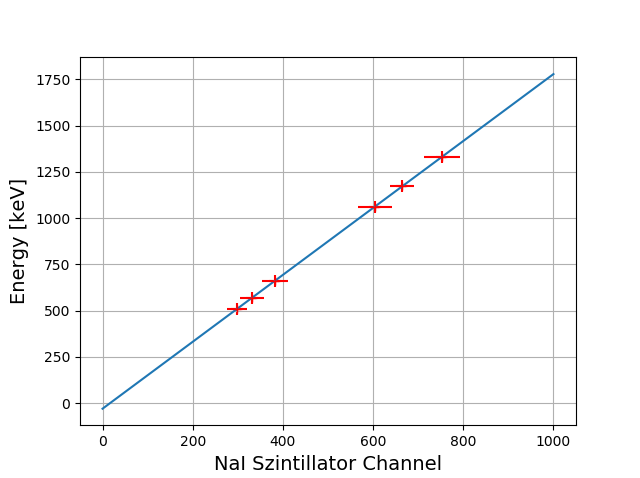
\includegraphics[width=\linewidth]{pictures/szin_kali.png}
  \caption{Calibration curve of the NaI scintilator}
  \label{szin_kali}
\end{figure}
Fitparameters were calculated to a slope of $m = 1.8084 \pm 0.0041$ and an intercept of $n = -29.6 \pm 2.2$
Putting this all together gives us for the scintilator the calibration curve:
\begin{equation}
E(K) = [(1.8084 \pm 0.0041) \cdot K - (29.6 \pm 2.2)]  \text{keV}
\end {equation}

\clearpage

\subsection{Energy Resolution}

With the calibration curve, we now looked into the energy resolution of the scintilator.
Just like for the HGPE detector, the resolution should be dependant on:
\begin{itemize}
\item an electronic noise term $a$
\item a term for statistical fluctioations $b$
\item a term for inhomgenieties in the detector $c$
\end{itemize}
For the NaI detector, the inhomogeneties should be of lesser concern for the uncertainty, which means that we will neglect $c$.
This modifies the theoretical function to:
\begin{equation}
\frac{\Delta E}{E} = \frac{\sqrt{a + bE }}{E}
\label{szin_resolution}
\end{equation}
As uncertainty for the energy ($\Delta E$) we used again the FHWM calculated in Tab. \ref{szin_peaks}.
Plotting $\frac{\Delta E}{E}$ und fitting according to Eq. \ref{szin_resolution} gave us Fig. \ref{szin_res}.

\begin{figure}[h]
  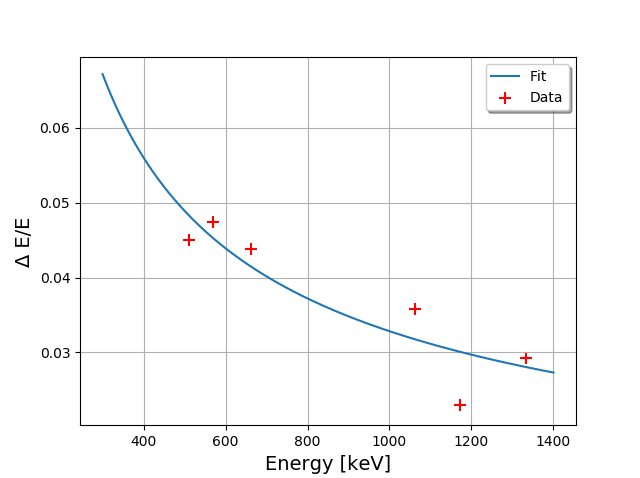
\includegraphics[width=\linewidth]{pictures/szin_res.png}
  \caption{Energy reslution of the NaI scintilator}
  \label{szin_res}
\end{figure}
With the fitting contsants: $a = 118 \pm 16$ and $b = 0.96 \pm 0.14$.
In Fig. \ref{szin_res} we can see, that the points have a pretty high deviation from the fit, yet in generell the function seems to work with the data.
This might have to do with the in generel high deviation of this scintilator.
Some more points for the fit should have made the result better.

\clearpage
